%Dokumentklasse
%\documentclass[a4paper,12pt]{scrreprt}
\documentclass[a4paper,12pt,oneside,pointlessnumbers]{scrbook}
\usepackage[left= 2.5cm,right = 2cm, bottom = 4 cm]{geometry}
%\usepackage[onehalfspacing]{setspace}
% ============= Packages =============

% Dokumentinformationen
\usepackage[
	pdftitle={Dokumentation},
	pdfsubject={},
	pdfauthor={Michael Stroh, Daniel Schwenk},
	pdfkeywords={},	
	%Links nicht einrahmen
	hidelinks
]{hyperref}


% Standard Packages
\usepackage[utf8]{inputenc}
\usepackage[ngerman]{babel}
\usepackage[T1]{fontenc}
\usepackage{graphicx, subfig}
\graphicspath{{img/}}
\usepackage{fancyhdr}
\usepackage{lmodern}
\usepackage{color}
\usepackage{pdfpages} 
\usepackage{listings}
\usepackage{adjustbox}
\usepackage{multirow}
\usepackage[printonlyused]{acronym}
\usepackage[nomain,acronym,xindy,toc]{glossaries}

% zusätzliche Schriftzeichen der American Mathematical Society
\usepackage{amsfonts}
\usepackage{amsmath}


%nicht einrücken nach Absatz
%\setlength{\parindent}{0pt}


% ============= Kopf- und Fußzeile =============
\pagestyle{fancy}
%
\lhead{}
\chead{}
\rhead{\slshape \leftmark}
%%
\lfoot{}
\cfoot{\thepage}
\rfoot{}
%%
\renewcommand{\headrulewidth}{0.4pt}
\renewcommand{\footrulewidth}{0pt}

% ============= Package Einstellungen & Sonstiges ============= 
%Besondere Trennungen
\hyphenation{De-zi-mal-tren-nung}


% ============= Dokumentbeginn =============

\begin{document}
%Seiten ohne Kopf- und Fußzeile sowie Seitenzahl
\pagestyle{empty}



\begin{figure}%
    \centering
    \subfloat{{
\includegraphics[scale=0.35]{img/hs_weingarten.png} }}%
    \qquad \qquad \qquad \qquad \qquad \qquad
    \subfloat{{
\includegraphics[scale=0.22]{img/ai.jpg} }}%
\end{figure}


\begin{center}
\begin{tabular}{p{\textwidth}}

\\

\begin{center}
\LARGE{\textsc{
Dokumentation \\
}}
\end{center}

\\


\begin{center}
\large{zur Vorlesung Systemadministration \\
im Bachelor Studiengang Angewandte Informatik \\}
\end{center}

\\

\begin{center}
\large{Wintersemester 2016 / 2017 \\
 bei Herr Prof. Dr. Eggendorfer\\}
\end{center}

\\

\begin{center}
\huge{\textbf{Umsetzung von Honeypots \\
auf Basis eines Raspberry Pis}} \\

\end{center}


\\

\\


\begin{center}
\large{\textbf{Michael Stroh}} \\
\small{Matrikelnr. 24972}
\end{center}

\begin{center}
\large{\textbf{Daniel Schwenk}} \\
\small{Matrikelnr. 24961}

\end{center}

\\

\\

\begin{center}
\large{05. Oktober 2016}
\end{center}




\end{tabular}
\end{center}

% Beendet eine Seite und erzwingt auf den nachfolgenden Seiten die Ausgabe aller Gleitobjekte (z.B. Abbildungen), die bislang definiert, aber noch nicht ausgegeben wurden. Dieser Befehl fügt, falls nötig, eine leere Seite ein, sodaß die nächste Seite nach den Gleitobjekten eine ungerade Seitennummer hat. 
\cleardoubleoddpage

\pagestyle{fancy}

\pagenumbering{roman} % römische nummerieung für Abbildungsverzeichnis + Tabellenverzeichnis


%Inhaltsverzeichnis
\tableofcontents

%\newpage % new page, damit nummerierung passt ...
% Abbildungsverzeichnis in Inhaltsverzeichnis aufnehmen
%\addcontentsline{toc}{chapter}{Abbkürzungsverzeichnis}
%\include{001_abkuerzungsverzeichnis}

%\newpage % new page, damit nummerierung passt ...
% Abbildungsverzeichnis in Inhaltsverzeichnis aufnehmen
%\addcontentsline{toc}{chapter}{Abbildungsverzeichnis}
%Verzeichnis aller Bilder
%\listoffigures

%\newpage % new page, damit nummerierung passt ...
% Tabellenverzeichnis in Inhaltsverzeichnis aufnehmen
%\addcontentsline{toc}{chapter}{Tabellverzeichnis}
%Verzeichnis aller Tabellen
%\listoftables


% pagestyle für gesamtes Dokument aktivieren
\pagestyle{fancy}

\pagenumbering{arabic}
\chapter{Einleitung}
\label{ch:einleitung}

Das Internet und die Digitalisierung, die in alle Lebensbereiche Einzug hält, verändern Gesellschaft, Wirtschaft und Kultur. Egal ob im privaten oder beruflichen Umfeld, ständig sind wir von Computern in Form von Arbeitsgeräten, Smartphones oder anderen Geräten umgeben. Diese Verbreitung sowie die Vernetzung von Geräten untereinander wird in den nächsten Jahren im Zuge der "`Internet-der-Dinge-Evolution"' weiter drastisch zunehmen.\\


Ein oft vernachlässigter Aspekt ist hierbei das Thema "`IT-Sicherheit"'. Keine Software ist frei von Fehlern und Sicherheitslücken. Falsch konfigurierte Dienste und Software, die nicht regelmäßig aktualisiert wird, sind ein leichtes Ziel für Angreifer. Durch die zunehmende Vernetzung wird das Thema IT-Sicherheit in Zukunft weiter an Bedeutung gewinnen.\\

Um eine Infrastruktur, egal ob im privaten oder geschäftlichen Bereich, vor möglichen Angriffen zu schützen bedarf es eines immer größeren Aufwandes.



\section{Motivation}
\label{sec:Motivation}

Die Gewährleistung der IT-Sicherheit ist mittlerweile eine immens wichtige, wenn nicht sogar die wichtigste Anforderung an eine intakte IT-Infrastruktur. Entsprechend sollte ein Systemadministrator über ein breites Spektrum an Wissen im Bereich der IT-Sicherheit besitzen sowie in der Lage sein, mögliche Angriffsszenarien frühzeitig zu erkennen.\\


Das Konzept eines Honeypots, also einen potentiellen Angreifer nicht nur vor eigentlich wichtigen System fernzuhalten, sondern auch noch von seinem Wissen zu profitieren, stellt dabei einen hochspannenden Ansatz dar. 
Dieser Ansatz soll dem Projektteam helfen, Wissen über mögliche Angriffsszenarien und Vorgehensweisen zu erlangen, um so die Sicherheit von bestehenden und zukünftigen Infrastrukturen gewährleisten zu können.

\newpage


\section{Ziele}
\label{sec:Ziele}

Ziel dieser Arbeit ist es, ein System zu entwickeln, das als Honeypot dient. Dieser Honeypot soll eingesetzt werden, um Einblicke in die Vorgehensweise eines Angreifers zu bekommen. 
Das System stellt dazu ein vermeintlich leicht angreifbaren Webserver sowie SSH-Server dar.\\


Jegliche Zugriffe und Aktivitäten die ein Angriff hinterlässt werden protokolliert und ausgewertet. Das hierbei gewonnene Wissen soll in Form von IT-Sicherheitsmaßnahmen in bestehende und künftige IT-Infrastrukturen einfließen.

\begin{itemize}
\item Primärziel: einsatzfähige(r) Honeypot(s) - sicher, authentisch und lehrreich
\end{itemize}




\section{Eigene Leistung}
\label{sec:Eigene Leistung}

Der Hauptbestandteil dieses Projekts liegt in der Inbetriebnahme und Bereitstellung eines Honeypots, sowie die Integration desselben in eine für einen potentiellen Angreifer authentisch erscheinenden Umgebung. Dabei liegt das Hauptaugenmerk darauf, die Sicherheit des Systems zu gewährleisten. Die Dokumentation der Infrastruktur, der stattgefundener Angriffe sowie deren Auswertung stellen einen wichtigen Bestandteil dar. Dieses Wissen dient dem Projektteam zukünftig zur Absicherung von IT-Infrastruktur.

\begin{itemize}
\item Bereitstellung einer authentischen Umgebung für den Honeypot
\item Gewährleistung der Sicherheit für das eigene und das globale Netz
\item Inbetriebnahme des Honeypots selbst
\item Auswertung von Log-Files et cetera
\item Dokumentation von Honeypot inklusive Umgebung, Angriffsphase und Ergebnisse
\end{itemize}



\chapter{Anforderungen}
\label{ch:Anforderungen}

Die Anforderungen an das Honeypot-System werden in Muss-, Kann- und Soll-Kriterien unterteilt.


\section{Muss-Kriterien}
\label{sec:Muss-Kriterien}
\begin{itemize}
\item Honeypot ist über das Internet erreichbar
\item Honeypot darf keinerlei Gefahr für andere Systeme darstellen
\item Honeypot muss jederzeit deaktivierbar sein
\item Angreifer darf keinerlei Möglichkeit zur Interaktion mit dem Host-Betriebssystem haben
\item Angreifer darf keine bzw. nur gefälschte Antworten auf Anfragen erhalten
\item Honeypot muss mindestens einen, besser jedoch mehrere Dienste, wie beispielsweise HTTP, SSH oder FTP, simulieren/anbieten
\item Honeypot muss ein realistisch wirkendes Angriffsziel darstellen
\item Angriffe werden geloggt
\item Ein- und ausgehender Netzwerkverkehr muss (überwacht und) geloggt werden 
\item Protokollierte Daten dürfen durch Angreifer nicht verändert werden können

\end{itemize}

\newpage

\section{Soll-Kriterien}
\label{sec:Soll-Kriterien}
\begin{itemize}
\item Automatische Benachrichtigung, wenn System angegriffen wird
\item Protokollierung und ggf. Forwarding von Log-Files dürfen für den Angreifer nicht sichtbar sein
\item Automatisierte Auswertung von Logdaten
\item Logdateien / ausgewertete Daten werden automatisch separat gespeichert (extra System, Cloud-Speicher)
\end{itemize}


\section{Kann-Kriterien}
\label{sec:Kann-Kriterien}
\begin{itemize}
\item Geringer Stromverbrauch von Honeypot-System
\item Kostengünstiger Versuchsaufbau
\item Reverse DNS-Lookup von Angreifer-IP-Adresse(n)
\item Simulation weiterer Geräte (Router, Firewall, PC)
\item Honeypot simuliert offenes WLAN-Netz / Fake-Access-Point
\end{itemize}




\chapter{Gantt-Diagramm}
\label{sec:Gantt-Diagramm}

\begin{center}
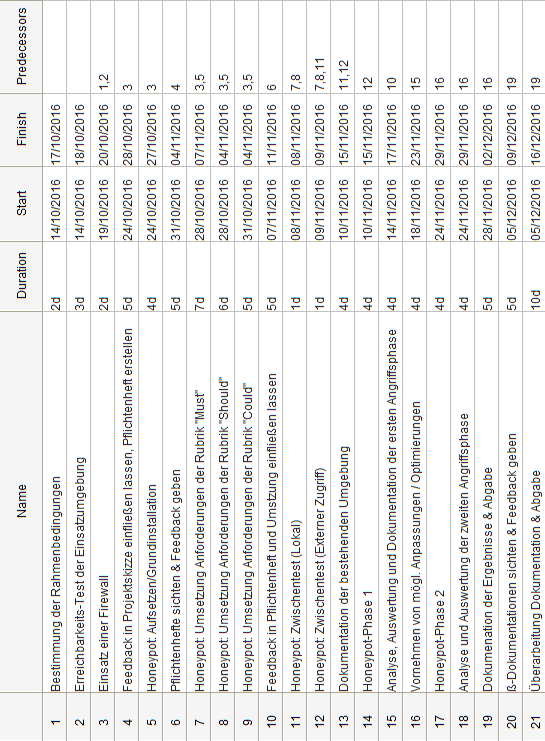
\includegraphics[scale=0.78]{img/gantt_tasks.png}
\end{center}

\newpage

\begin{center}
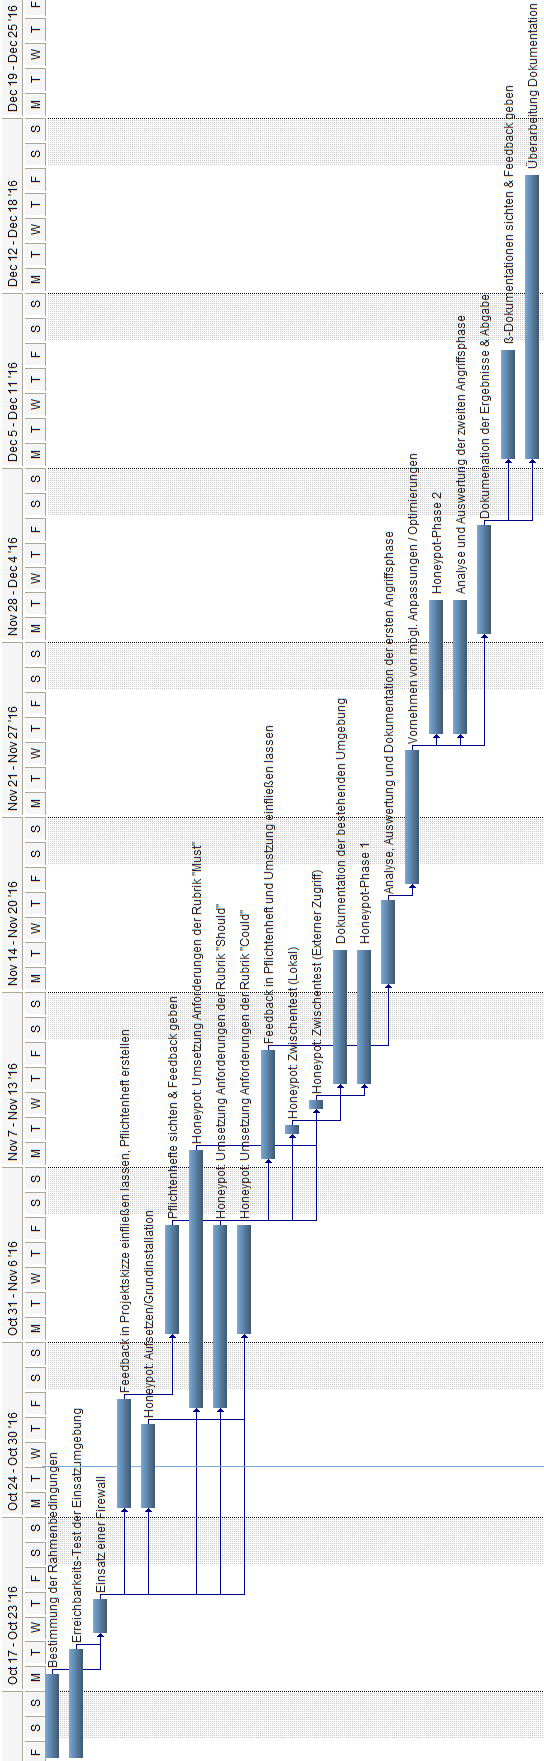
\includegraphics[scale=0.50]{img/gantt_diagram.png}
\end{center}

\chapter{Marktanalyse}
\label{ch:Marktanalyse}

Eine Marktanalyse zeigt, dass eine Vielzahl an verschiedenen Honeypot-Paketen, Skripten und Konfigurationen mit sehr unterschiedlichen Eigenschaften verfügbar sind. Darunter befinden sich sowohl kommerzielle als auch freie Lösungen.

\section{HoneyDrive}
\label{sec:HoneyDrive}
Mit HoneyDrive existiert eine Honeypot-Linux-Distribution auf Basis von Xubuntu Desktop 12.04.04 LTS. Diese Linux-Distribution bringt 10 vorinstallierte und vorkonfigurierte Honeypot-Pakete wie Kippo SSH Honeypot, Glastopf Web Honeypot oder Amun Malware Honeypot mit. Die Distribution wird als OVA-Datei angeboten und kann so unter einer Virtualisierungssoftware ausgeführt werden. Neben den vorinstallierten Honeypot-Paketen sind des weiteren unter anderem ein Web- und Datenbankserver sowie wie PHPMyAdmin vorinstalliert.
Diese Linux-Distribution ermöglicht so einfach und schnell ein Honeypot-System aufzusetzen.\\

Das große Manko ist hier der veraltete Software-Stand. Die letzte Aktualisierung fand im Jahre 2014 statt. Dies, sowie der Overhead an vorinstallierten und vorkonfigurierten Diensten, birgt die Gefahr, dass ein potenzieller Angreifer über eine Lücke das Hostsystem kompromittieren oder übernehmen kann.

\section{Kippo}
\label{sec:Kippo}
Kippo ist ein SSH-Honeypot, entworfen um Bruteforce-Attacken sowie die komplette Interaktion des Angreifers mit der Shell zu protokollieren.\\
Um der Anforderung der automatischen Benachrichtigung des Projektteams bei einem Angriff gerecht zu werden, gilt es Logdateien automatisiert zu analysieren und auszuwerten. Wird ein Bruteforce-Angriff erkannt, wird das Projektteam via Email benachrichtigt. Diese Anforderung kann Kippo ohne Anpassungen nicht leisten.\\

Ein wesentlicher Nachteil von Kippo ist die Tatsache, dass sich Tools zu seiner Erkennung im Umlauf befinden. Entsprechend versierte Angreifer werden Kippo daher frühzeitig erkennen.

\section{Honeyd}
\label{sec:Honeyd}
Honeyd wird von unix-artigen Betriebssystemen unterstützt. Er ist ein Daemon, der virtuelle Hosts in einem Netzwerk erzeugt. Diese Hosts können das Vorhandensein spezieller Betriebssysteme und Services simulieren, indem sie mit authentischen Antwortpaketen auf etwaige Anfragen, insbesondere Fingerprint-Pakete reagieren. Honeyd eignet sich besonders für die Ablenkung eines Angreifers und die Verschleierung der wirklichen Infrastruktur. Ebenso  dient er als Warnsystem, da jeder Zugriffsversuch auf einem der durch Honeyd erzeugten Hosts ein Hinweis auf unerwünschte Aktivitäten innerhalb der Infrastruktur darstellt.\\

Honeyd eignet sich nicht ohne Weiteres für die Aufzeichnung komplexerer Angriffe, insbesondere solcher, die auf dem System selbst stattfinden, bietet jedoch die Möglichkeit weitere Geräte zu simulieren und somit zur Authentizität der Infrastruktur des Projektteams beizutragen.

\section{Glastopf}
\label{sec:Glastopf}

Glastopf ist ein als Webserver getarnter Honeypot. Dieses System nutzt den Umstand, dass viele Angreifer unter Zuhilfenahme von Suchmaschinen nach Schwachstellen auf Webservern suchen, indem es sich selbst bei den gängigsten Vertretern registriert. Dabei wird Fläche für gängige, webbasierte Angriffe wie SQL-Injections, Remote-Code-Execution, File-Inclusion et cetera, geboten. Von einem Angreifer eingeschleuster Code, wird in einer Sandbox ausgeführt. Alle Verbindungen und Angriffsversuche werden geloggt und in einer Datenbank protokolliert.\\

Durch die Mithilfe von Webcrawlern ist es mit Glastopf möglich für die eigenen Schwachstellen Reklame zu betreiben und somit in kürzerer Zeit eine größere Menge an Angriffen auf das System zu lenken. Die optische Aufmachung der Glastopf-Startseite trägt allerdings dazu bei, dass Angriffe in sehr hohem Anteil nur automatisiert und kaum oder gar nicht in individuell gezielter Form stattfinden werden.

%Literaturverzeichnis
%\addcontentsline{toc}{chapter}{Literaturverzeichnis}
%\bibliographystyle{unsrtdin}
%\bibliography{Literatur}

%\include{09_anhang}

%\section*{Selbst"andigkeitserkl"arung}
%\addcontentsline{toc}{section}{Selbst"andigkeitserkl"arung}
\thispagestyle{empty}


Ich versichere, dass ich die vorliegende Dokumentation selbständig verfasst und keine anderen als die angegebenen Quellen und Hilfsmittel benutzt habe.\\
\setlength{\parindent}{0pt}\\
Die Tabellen, Abbildungen oder Listings in dieser Arbeit sind von mir selbst erstellt worden oder mit einem entsprechenden Quellennachweis versehen.

\vspace{0.5cm}\noindent\hspace{1.5cm}

Weingarten, den 02. Dezember 2016

\vspace{1cm}\noindent\hspace{1.5cm}

Unterschrift: \noindent\hspace*{10mm}...........................\hspace*{10mm}...........................\\
\noindent\hspace*{34.5mm}Michael Stroh\hspace*{16.2mm}Daniel Schwenk


\newpage
\thispagestyle{empty}
\chapter*{ }
\thispagestyle{empty}

\end{document}
